\documentclass[12pt]{report}
\usepackage{amssymb}
\usepackage{caption}
\usepackage{fancybox}
\usepackage{wasysym}
\usepackage{geometry} % Page Dimensions
\geometry{a4paper, total={170mm,260mm}, left=20mm, top=20mm}
\usepackage{fontspec} % Γραμματοσείρες
\usepackage{xcolor} % Χρώματα
\usepackage{colortbl} % Χρωματισμός πινάκων
\usepackage{tabularx} % Πίνακες με μεταβλητό πλάτος στηλών
\usepackage{tabularray} % Πίνακες με πιο ευέλικτη διαμόρφωση
\usepackage{multicol} % Πολλαπλές στήλες (όχι για μαθηματικά)
\usepackage{hyperref} % Σύνδεσμοι στο pdf
\UseTblrLibrary{booktabs}
\usepackage{amstex} % Επιπλέον μαθηματικά εργαλεία
\usepackage{amsmath} % Μαθηματικά εργαλεία
\usepackage{tcolorbox} % Μορφοποίηση πλαισίων
\usepackage{titlesec} % Μορφοποίηση τίτλων κεφαλαίων
\usepackage{setspace} % Διάστιχο
\usepackage[greek]{babel} % Ελληνική γλώσσα
\usepackage{indentfirst} % Εσοχή πρώτης παραγράφου
\usepackage{fancyhdr} % Κεφαλίδες και υποσέλιδα
\usepackage{forest} % Δημιουργία δέντρων
\usepackage{graphicx} % Διαχείριση εικόνων
\usepackage{enumitem} % Διαμόρφωση λιστών
\usepackage{listings} % Block κώδικα
\usepackage{arabicore} %
\usepackage{booktabs} % πίνακες
\usepackage{titleps} % επικεφαλίδες και υποσέλιδα
\usepackage{biblatex} % διαχείριση βιβλιογραφίας
\usepackage{lstmisc} %
\usepackage{tikz}

\graphicspath{ {./img/} }
%\usepackage[fontsize=13pt]{fontsize}

\setmainfont{Conduit ITC Hel Light}
\newfontfamily\fontDin{CF Din Condensed}
    \newenvironment{Din}{\fontDin}{\par}
\newfontfamily\fontDinLight{CF Din Light Condensed}
    \newenvironment{Din Light}{\fontDinLight}{\par}
\newfontfamily\fontDinMedium{CF Din Medium Condensed}
    \newenvironment{Din Medium}{\fontDinMedium}{\par}
%\newfontfamily\fontCode{Courier New}
    %\newenvironment{Code}{\fontCode}{\par}
\setmonofont[Scale=0.8]{Courier New}
\newfontfamily\fontTimes{Times New Roman}
    \newenvironment{Times}{\fontTimes}{\par}

\newfontfamily\headingfont[]{CF Din Medium Condensed}

\addto\captionsgreek{% Replace "english" with the language you use
  \renewcommand{\contentsname}%
    {ΠΕΡΙΕΧΟΜΕΝΑ}%
}

\newtcolorbox{headerdark}{colback=darkgray, boxrule=0pt,arc=0pt, boxsep=12pt,left=2pt,right=2pt,leftrule=0pt}
\newtcolorbox{headerlight}{colback=gray!50, boxrule=0pt,arc=0pt, boxsep=2pt,left=2pt,right=2pt,leftrule=0pt}
\newtcolorbox{graycomment}{colback=gray!25, boxrule=0pt,arc=0pt, boxsep=2pt,left=2pt,right=2pt,leftrule=1pt, grow to left by=-28pt,  grow to right by=-28pt}

% Το στιλ των νέων κεφαλαίων/sectionσ
\titleformat{\chapter}[block]
    {\color{black} \fontDin \large } % global formatting (number and title)
    {\color{white} \fontDin \colorbox{black!90} {\hspace{7pt}\thechapter\hspace{7pt}}} % label: number and its formatting
    {} % spacing between number and title
    {\colorbox{gray!25}} % optional (content between number and title)
\titlespacing*{\chapter}
   {0pt}{1em}{0.4em}  % left before after
\titleclass{\chapter}{straight}

\titleformat{\section}[block]
    {\color{black} \fontDinLight \large} % global formatting (number and title)
    {\color{white} \fontDin \colorbox{black!90} {\hspace{5pt}\thesection\hspace{5pt}}} % label: number and its formatting
    {} % spacing between number and title
    {\colorbox{gray!25}} % optional (content between number and title)
\titlespacing*{\section}
   {0pt}{1em}{0.4em}  % left before after

\titleformat{\subsection}[block]
    {\fontDinLight \large} % global formatting (number and title)
    {\fontDin\colorbox{gray!25} {\hspace{5pt}\thesubsection\hspace{5pt}}} % label: number and its formatting
    {\hspace{10pt}} % spacing between number and title
    {} % optional (content between number and title)
\titlespacing*{\subsection}
   {0pt}{1em}{0.4em}  % left before after

%% Setting for the column separator
%\colorlet{shadecol}{black!20}
%\setlength\columnsep{12pt}
%\makeatletter   % This change vertical bar to a dotted line
%\newcommand{\latexcolumnseprulecolor}{\color{shadecol}}
%\renewcommand\dotfill[1][0.4em]{%
%  \leavevmode\cleaders\hb@xt@ #1{\hss .\hss}\hfill\kern\z@}
%\patchcmd{\@outputdblcol}%
%  {\vrule\@width\columnseprule}%
%  {\rotatebox{90}{\parbox{\textheight}{\dotfill[0.3em]}}}%
%  {}{}
%\makeatother
%
%% Command to render shaded heading
%\newsavebox\labbox
%\NewDocumentCommand\shadedsec{O{1.5\baselineskip} O{0.33\dimexpr#1} m}{%
%  \sbox\labbox{%
%    \colorbox{black!80}{%
%      \textcolor{white}{\hspace{0.5em}#3\hspace{0.5em}}}}
%  \addvspace{#1}
%  \noindent%
%  \nopagebreak%
%  \usebox\labbox
%  {\color{shadecol}\rule[-\fboxsep]{\dimexpr\columnwidth-\wd\labbox}{\dimexpr\ht\labbox+\fboxsep}}%
%  \vspace{#2}\par}


% Ρύθμση αλλαγής γραμμής
\tolerance=1
\emergencystretch=\maxdimen
\hyphenpenalty=10000 % Για να μην κάνει συλλαβισμό στις λέξεις
\hbadness=10000

% Αλλαγή απόστασης μεταξύ παραγράφων
\setlength{\parskip}{6pt}

% Ρύθμιση Headers/Footers
\pagestyle{fancy}
\renewcommand{\headrulewidth}{0pt}
\fancyhead{}\fancyfoot{}
\fancyhead[R]{\fontDinLight ΑΛΕΞΑΝΔΡΟΣ ΞΙΑΡΧΟΣ \(\cdot\) 1059619\hspace{10pt}\colorbox{darkgray}{\color{white}\fontDin\thepage}}

% Συνεχόμενη αρίθμηση ανά chapters
\counterwithout{footnote}{chapter}

% Για γραμμές κώδικα
\lstdefinestyle{mystyle}{
    backgroundcolor=\color{gray!10},
    keywordstyle=\bf\ttfamily,
    numberstyle=\tiny\color{darkgray},
    basicstyle=\ttfamily\footnotesize,
    breakatwhitespace=false,
    breaklines=true,
    captionpos=b,
    showstringspaces=false,
    keepspaces=true,
    numbers=left,
    numbersep=5pt,
}
\lstset{style=mystyle}

\usepackage{float} % Allows for more flexible positioning of floats σε πίνακες πχ
\restylefloat{table}

\endinput


\begin{document}

    \begin{titlepage}
        \centering

        \renewcommand{\arraystretch}{1.1} % Increase row height
        \begin{tabularx}{\textwidth}{@{}m{0.9\textwidth}X@{}}
            \centering \raggedleft \cellcolor{lightgray!25} Αλέξανδρος Ξιάρχος\\ {\footnotesize st1059619@ceid.upatras.gr} & \centering\cellcolor{darkgray}\fontDin \raisebox{-1pt}{\color{white}1059619 \\}
        \end{tabularx}

        \vspace*{12em}
        \begin{headerlight}
            \begin{Din}
                \centering
                {ΠΑΝΕΠΙΣΤΗΜΙΟ ΠΑΤΡΩΝ \(\cdot\) ΤΜΗΜΑ ΜΗΧΑΝΙΚΩΝ Η/Υ ΚΑΙ ΠΛΗΡΟΦΟΡΙΚΗΣ}
            \end{Din}
        \end{headerlight}

        \begin{headerdark}
            \begin{Din Medium}
                \centering
                \huge \textcolor{white}{ΕΙΣΑΓΩΓΗ ΣΤΗ ΒΙΟΠΛΗΡΟΦΟΡΙΚΗ}
            \end{Din Medium}
        \end{headerdark}

        \begin{headerlight}
            \begin{Din}
                \centering
                ΠΡΩΤΟ ΣΥΝΟΛΟ ΑΣΚΗΣΕΩΝ \(\cdot\) 2023\(\textendash\)2024
            \end{Din}
        \end{headerlight}

        \vspace*{10em}

    \end{titlepage}

    \tableofcontents
    \pagebreak

%   ===================================================================================================================

    \chapter{ΕΡΩΤΗΜΑ 1}

    \section{ΕΡΓΑΛΕΙΑ ΓΙΑ ΧΕΙΡΙΣΜΟ ΠΡΟΒΛΗΜΑΤΩΝ ΒΙΟΠΛΗΡΟΦΟΡΙΚΗΣ}
    \chapter{ΕΡΩΤΗΜΑ 2}
    Χρησιμοποιούμε τις εξής αλυσίδες φεριττίνης:
    \begin{graycomment} \footnotesize
    \begin{verbatim}
>AAH13928.1 Ferritin, light polypeptide [Homo sapiens]
    MSSQIRQNYSTDVEAAVNSLVNLYLQASYTYLSLGFYFDRDDVALEGVSHFFRELAEEKREGYERLLKMQNQRGGRALFQ
    DIKKPAEDEWGKTPDAMKAAMALEKKLNQALLDLHALGSARTDPRLCDFLETHFLDEEVKLIKKMGDHLTNLHRLGGPEA
    GLGEYLFERLTLKHD
>NP_001126850.1 ferritin light chain [Pongo abelii]
    MSSQIRQNYSTDVEAAVNSLVNMYLQASYTYLSLGFYFDRDDVALEGVSHFFRELAEEKREGYERLLKMQNQRGGRALFQ
    DIKKPAEDEWGKTPDAMKAAMALEKKLNQALLDLHALGSAHTDPHLCDFLETHFLDEEVKLIKKMGDHLTNLHRLGGPEA
    GLGEYLFERLTLKHD
>XP_063672238.1 ferritin light chain-like [Pan troglodytes]
    MFWQFGGPAGLSLASTVFGRNRSGDSLPASDRPPISSPLATSGTIFSAISCFWDLPAPFLWLAPSCQPTMSSQIRQNYST
    DVEAAVNSLVNLYLQASYTYLSLGFYFDRDDVALEGVSHFFRELAEEKREGYERLLKMQNQRGGRALFQDIKKPAEDEWG
    KTPDAMKAAMALEKKLNQALLDLHALGSAHTDPHLCDFLETHFLDEEVKLIKKMGDHLTNLHRLGGPEAGLGEYLFERLT
    LKHD\end{verbatim}
    \end{graycomment}

    \section{ΣΤΟΙΧΙΣΗ ΑΚΟΛΟΥΘΙΩΝ}
        Για τη στοίχιση των ακολουθιών χρησιμοποιούμε το εργαλείο T-COFFEE \cite{TCoffee}.

        \begin{center} \noindent
            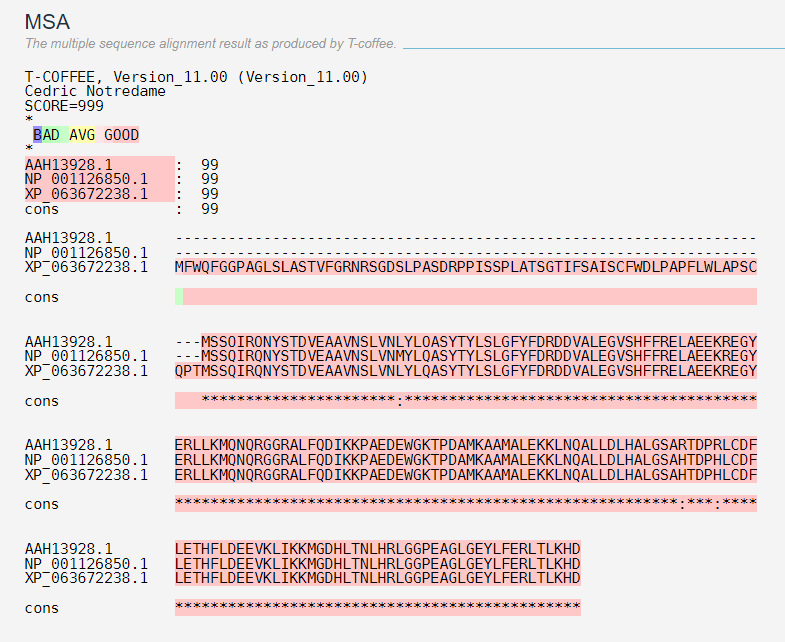
\includegraphics[scale=0.75]{img/T-Coffee}
        \end{center}

        Βλέπουμε πως υπάρχει μια πολύ καλή βαθμολογία (99), το οποίο σημαίνει πως υπάρχει μεγάλη ομοιότητα ανάμεσα στις ακολουθίες.

    \section{ΣΥΓΚΡΙΣΗ ΔΟΜΩΝ}

        \begin{center} \noindent
            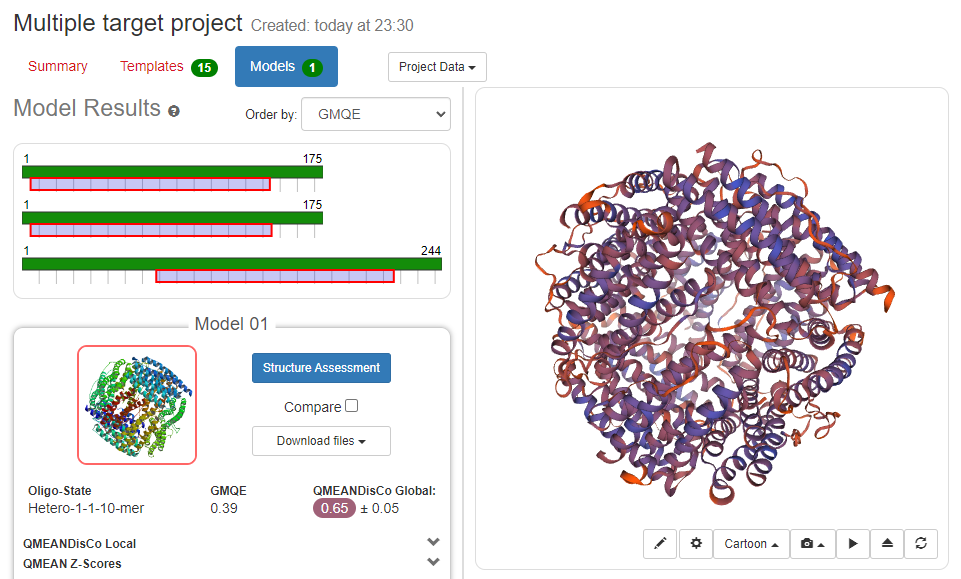
\includegraphics[scale=0.7]{img/swiss-modeller}
        \end{center}

            Αφού εξάγουμε το αρχείο \texttt{.pdb} μέσω του swiss-modeller, συγκρίνουμε τις δομές χρησιμοποιώντας το Dali.

    \begin{graycomment} \footnotesize
    \begin{verbatim}
1287:  8jb0-F 15.3  2.1  128   161   13   MOLECULE: BACTERIOFERRITIN;
1288:  8jb0-T 15.3  2.0  128   162   14   MOLECULE: BACTERIOFERRITIN;
1289:  8jb0-S 15.3  2.1  129   161   13   MOLECULE: BACTERIOFERRITIN;
1290:  2pyb-A 15.3  1.9  131   151    7   MOLECULE: NEUTROPHIL ACTIVATING PROTEIN;
1291:  6zlq-Z 15.2  2.3  136   174   75   MOLECULE: FERRITIN;
1292:  6zlq-G 15.2  2.3  136   174   75   MOLECULE: FERRITIN;
1293:  6job-B 15.2  2.4  137   172   50   MOLECULE: FERRITIN HEAVY CHAIN;
1294:  6job-A 15.2  2.4  137   172   50   MOLECULE: FERRITIN HEAVY CHAIN;
1295:  5obb-F 15.2  2.4  136   174   49   MOLECULE: FERRITIN HEAVY CHAIN;
1296:  1xz1-A 15.2  2.4  137   168   82   MOLECULE: FERRITIN LIGHT CHAIN;\end{verbatim}
    \end{graycomment}
    \chapter{ΕΡΩΤΗΜΑ 3}

    Τα γενικευμένα δέντρα επιθεμάτων (generalized suffix trees) επιτρέπουν την αποθήκευση και την αναζήτηση πολλαπλών συμβολοσειρών, εν αντιθέσει με τα δέντρα επιθεμάτων (suffix trees) που αφορούν μια συγκεκριμένη συμβολοσειρά.
    Πρόκειται για μια \textbf{στατική δομή δεδομένων}, μιας και κατασκευάζεται για κάποιες συγκεκριμένες συμβολοσειρές που ορίζονται εξ' αρχής.
    Ως αποτέλεσμα, η δομή δεν έχει σχεδιαστεί για να δέχεται εύκολα τροποποιήσεις, όπως είναι η εισαγωγή νέων συμβολοσειρών ή η διαγραφή υπάρχοντων. Συγκεκριμένα:

    \section{ΠΡΟΒΛΗΜΑΤΑ ΣΤΑΤΙΚΩΝ ΔΕΝΤΡΩΝ}
        Για να μπορέσει να εισαχθεί μια νέα συμβολοσειρά στο γενικευμένο δέντρο επιθεμάτων, είναι απαραίτητη η ανακατασκευή ολόκληρου του δέντρου μιας και άλλαξε η είσοδος.

        Έτσι όλα τα υπάρχοντα μονοπάτια --που αναπαριστούν τα υπάρχοντα επιθέματα-- χρειάζεται να ανανεωθούν για να συμβαδίζουν με τις αλλαγές της εισόδου.
        Παρόμοια ανανέωση απαιτείται και με διαγραφή κάποιας συμβολοσειράς, αφού τροποποιείται και πάλι η είσοδος του δέντρου.

        Η αναδιάρθρωση των μονοπατιών από την αρχή μετά από κάθε εισαγωγή και διαγραφή δεν είναι αποδοτική καθώς κάθε φορά είναι απαραίτητο να επαναυπολογιστεί ολόκληρο το δέντρο.

    \section{ΔΥΝΑΜΙΚΟΙ ΑΛΓΟΡΙΘΜΟΙ}
        Είναι σαφές ότι είναι απαραίτητος ένας δυναμικός τρόπος διαχείρισης της δομής, ώστε να μη χρειάζεται η ανακατασκευή όλων των μονοπατιών κάθε φορά που αλλάζει η είσοδος του δέντρου, αλλά παρά μόνο των μονοπατιών που επηρεάζονται.

        \subsection{Δυναμικό δέντρο επιθεμάτων του McCreight}
            Ο McCreight προτείνει έναν νέο αλγόριθμο \cite{McCreight_1976}, ο οποίος κατασκευάζει το δέντρο επιθεμάτων σταδιακά (Algorithm M):
            Ξεκινάει από τη ρίζα και το πρώτο χαρακτήρα της συμβολοσειράς.
            Για κάθε επόμενο χαρακτήρα επεκτείνει το δέντρο προσθέτοντας τα επιθέματα που ξεκινούν από αυτόν τον χαρακτήρα, με τελική πολυπλοκότητα \(O(n)\).
            Κατ' αυτόν τον τρόπο, δεν είναι απαραίτητη η πρότερη γνώση όλων των συμβολοσειρών, συντελώντας σε μια \textit{κάπως} δυναμική μορφή δέντρου, από την άποψη ότι δε χρειάζεται η πρωτύτερη γνώση ολόκληρης της εισόδου για να ξεκινήσει η εισαγωγή των επιθεμάτων.

        \subsection{Δυναμικό δέντρο επιθεμάτων των Choi - Lam}
            Οι Choi - Lam προτείνουν μια νέα δυναμική υλοποίηση για το δέντρο επιθεμάτων. \cite{Choi_Lam_1997}
            Κατά την εισαγωγή μιας νέας συμβολοσειράς, το δέντρο ψάχνει το μεγαλύτερο επίθεμα και μετά προσθέτει τα νέα επιθέματα κάνοντας τις απαραίτητες μεταβολές στις ακμές και στους κόμβους.
            Στην εισαγωγή χρησιμοποιείται μια ιδέα που παρουσίασε και ο McCreight, τα suffix links.

            Αντίστοιχα κατά τη διαγραφή μιας συμβολοσειράς \(s\), αναγνωρίζονται και διαγράφονται οι ακμές / επιθέματα που σχετίζονται με το \(s\) και ο αλγόριθμος ανανεώνει τις ετικέτες των φύλλων τους.
            Το αποτέλεσμα είναι σε κάθε περίπτωση να επανακατασκευάζεται το δέντρο ακέραια, επιτρέποντας τη δυναμική προσθήκη και διαγραφή συμβολοσειρών σε \(O(nlogA)\) χρόνο.

        \subsection{Online αλγόριθμος του Ukkonen}
            O Ukkonen προτείνει έναν νέο αλγόριθμο κατασκευής δέντρων επιθεμάτων σε γραμμικό χρόνο. \cite{Ukkonen_1995}
            Ο αλγόριθμος διαχειρίζεται την εισαγωγή και διαγραφή των συμβολοσειρών με έναν τρόπο που επιτρέπει την ανανέωση του δέντρου χωρίς να χρειάζεται η ανακατασκευή όλων των μονοπατιών.

            Για κάθε νέο χαρακτήρα που εισάγεται, ο αλγόριθμος ανανεώνει το δέντρο επιθεμάτων επεκτείνοντας τα υπάρχοντα επιθέματα με τον νέο χαρακτήρα.
            Όταν διαγράφεται μια συμβολοσειρά, ο αλγόριθμος διασχίζει το δέντρο για να εντοπίσει και να διαγράψει τους κόμβους που αντιστοιχούν στα επιθέματα του διαγραμμένου χαρακτήρα.
            Αυτά επιτυγχάνονται σε γραμμικό χρόνο.

        \subsection{LCP αλγόριθμος των Cole - Hariharan}
            Τέλος οι Cole - Hariharan προτείνουν έναν LCP (Longest Common Prefix) αλγόριθμο για το δέντρο επιθεμάτων, με \(O(\log n)\) χειρότερο χρόνο για εισαγωγές και διεγραφές. \cite{Cole_Hariharan_2005}

    \chapter{ΕΡΩΤΗΜΑ 4}
    Σκοπός είναι η εύρεση των μέγιστων multirepeats (συμβολοσειρά που εμφανίζεται πολλαπλές σειρές) σε μια συλλογή ακολουθιών: \cite{Bakalis_2006}
    \vspace{-10pt}
    \begin{center} \noindent
        \includegraphics[scale=0.4]{img/erwthma4_example}
    \end{center}

    \section{ΧΩΡΙΣ ΠΕΡΙΟΡΙΣΜΟΥΣ ΣΤΑ ΚΕΝΑ}
    Θα χρησιμοποιήσουμε γενικευμένο δέντρο επιθεμάτων στο οποίο κάθε κόμβος έχει δύο το πολύ παιδιά (binarizated).
    Διασχίζοντας το δέντρο από τα φύλλα προς τη ρίζα, περνάμε ταυτόχρονα από κόμβους με κοινό πατέρα.

    Έτσι για κάθε ζευγάρι των κόμβων \(v\) και \(w\) αναζητούνται multirepeats που δημιουργούνται από τα κοινά προθέματα των επιθεμάτων των κόμβων, και αν βρεθούν, συνενώνονται σε leaf lists.
    Τα leaf lists περιλαμβάνουν όλες τις εμφανίσεις των επιθεμάτων στο υποδέντρο που εξετάζουμε.
    Αυτές, συνενώνονται και αντιστοιχίζονται στον πατέρα κόμβο \(z\).
    Η διαδικασία επαναλαμβάνεται προς τα πάνω.

    \section{ΜΕ ΠΕΡΙΟΡΙΣΜΟΥΣ ΣΤΑ ΚΕΝΑ}
    Στην περίπτωση που υπάρχουν ειδικές συνθήκες στο μεσοδιάστημα ανάμεσα στις συμβολοσειρές που επαναλαμβάνονται (για παράδειγμα αν υπάρχει κάποιος περιορισμός των χαρακτήρων), ο αλγόριθμος πρέπει να διασφαλίσει τα τους περιορισμούς στα κενά:

    Πάλι διασχίζουμε το γενικευμένο binarized δέντρο επιθεμάτων από κάτω προς τα πάνω και περνάμε από ζευγάρια ακμών.
    Η διαφορά είναι πως πλέον ταξινομούμε τα leaf lists.
    Η ταξινόμηση είναι σημαντική, μιας και έτσι διασφαλίζεται η αποδοτική εύρεση δυνητικών συμβολοσειρών που ικανοποιούν τους περιορισμούς στα κενά που θέσαμε.
    Η υπόλοιπη διαδικασία είναι η ίδια με την προηγούμενη.
    \chapter{ΕΡΩΤΗΜΑ 5}
    \vspace{-10pt}
    \begin{center} \noindent
        \includegraphics[scale=0.5]{img/Erwthma5_Tree}
    \end{center}

    Έστω πρότυπο \(P\) και κείμενο \(T\).
    Ο μόνος αλγόριθμος που μπορεί να τρέξει realtime, δηλαδή σε \(O(n+m)\) χρόνο, όπου \(n\) ο συνολικός αριθμός χαρακτήρων του \(T\)
        και \(m\) το μήκος του προτύπου \(P\), είναι ο \textbf{Knuth-Morris-Pratt} αλγόριθμος.

    Εφαρμόζουμε τον αλγόριθμο αφού πρώτα διασχίσουμε το δέντρο, όπου για κάθε χαρακτήρα \(\in P \) ακολουθούμε τις ακμές που αντιστοιχούν σε αυτό.
    Μπορεί να χρησιμοποιηθεί κάποιος DFS αλγόριθμος για την εύρεση όλων των εμφανίσεων.
    \chapter{ΕΡΩΤΗΜΑ 6}

    \section{ΤΟΠΙΚΗ ΣΤΟΙΧΙΣΗ}

    \begin{table}[ht] \noindent\centering
        \resizebox{0.6\textwidth}{!}{
            \begin{tabular}{c|ccccccccccc}
       \bf{D} &   & \bf{G} & \bf{U} & \bf{G} & \bf{T} & \bf{T} & \bf{G} & \bf{T} & \bf{G} & \bf{G} \\
            \midrule
              & \colorbox{lightgray!25}{0} & \colorbox{lightgray!25}{0} & \colorbox{lightgray!25}{0} & \colorbox{lightgray!25}{0} & \colorbox{lightgray!25}{0} & \colorbox{lightgray!25}{0} & \colorbox{lightgray!25}{0} & \colorbox{lightgray!25}{0} & \colorbox{lightgray!25}{0} & \colorbox{lightgray!25}{0} \\
       \bf{T} & \colorbox{lightgray!25}{0} & 0 & 0 & 0 & 0 & 0 & 0 & 0 & 0 & 0 \\
       \bf{C} & \colorbox{lightgray!25}{0} & 0 & 0 & 0 & 0 & 0 & 0 & 0 & 0 & 0 \\
       \bf{G} & \colorbox{lightgray!25}{0} & 0 & 0 & 0 & 0 & 0 & 0 & 0 & 0 & 0 \\
       \bf{T} & \colorbox{lightgray!25}{0} & 0 & 0 & 0 & 0 & 0 & 0 & 0 & 0 & 0 \\
       \bf{G} & \colorbox{lightgray!25}{0} & 0 & 0 & 0 & 0 & 0 & 0 & 0 & 0 & 0 \\
       \bf{A} & \colorbox{lightgray!25}{0} & 0 & 0 & 0 & 0 & 0 & 0 & 0 & 0 & 0 \\
       \bf{A} & \colorbox{lightgray!25}{0} & 0 & 0 & 0 & 0 & 0 & 0 & 0 & 0 & 0 \\
       \bf{T} & \colorbox{lightgray!25}{0} & 0 & 0 & 0 & 0 & 0 & 0 & 0 & 0 & 0 \\
       \bf{T} & \colorbox{lightgray!25}{0} & 0 & 0 & 0 & 0 & 0 & 0 & 0 & 0 & 0 \\
            \end{tabular}}
    \end{table}


%    \pagebreak
%    \printbibliography
\end{document}
